\documentclass[twocolumn,10pt]{wmrDoc}

% --- Layout tightening (optional) ---
\usepackage{titlesec}
\titlespacing*{\section}{0pt}{1.5ex}{1.0ex}
\titlespacing*{\subsection}{0pt}{1.2ex}{0.8ex}
\titlespacing*{\subsubsection}{0pt}{1.0ex}{0.6ex}

\setlength{\textfloatsep}{8pt}
\setlength{\floatsep}{6pt}
\setlength{\intextsep}{6pt}
\setlength{\parskip}{2pt}

% --- Tables ---
\usepackage{booktabs}
\usepackage{tabularx}
\usepackage{array}
\usepackage{makecell}
\usepackage{placeins}   % \FloatBarrier
\usepackage{caption}    % captioned non-float blocks

\newcolumntype{Y}{>{\raggedright\arraybackslash}X}


% --- Figures / floats ---
\usepackage{graphicx}
\usepackage{float}        % enables [H]
\usepackage{dblfloatfix}  % improves float behavior in two-column

% --- TikZ for your diagram ---
\usepackage{tikz}
\usetikzlibrary{arrows.meta, positioning, shapes.geometric}
\usetikzlibrary{calc,positioning,arrows.meta,shapes.geometric}

% --- Caption ---
\usepackage[font=small,labelfont=bf]{caption}
\setlength{\abovecaptionskip}{2pt}
\setlength{\belowcaptionskip}{2pt}

% --- Hyperref should be last ---
\usepackage{hyperref}
\hypersetup{
  colorlinks=true,
  linkcolor=black,
  citecolor=black,
  urlcolor=black
}

\title{Security of Generative AI Systems: Prompt Injection and Model Misuse}

\author{Jana Khaled Beshir,
Sara Samy Elwakeel,
Sara Aly Ahmed,
Omar Khaled Ashour,
and Abdallah Sherif Tera}

\begin{document}
\maketitle

%%%%%%%%%%%%%%%%%%%%%%%%%%%%%%%%%%%%%%%%%%%%%%%%%%%%%%%%%%%%%%%%%%%%%%
\begin{abstract}
{\it
\textbf{Generative AI offers unprecedented new technologies with a rise of new threats to security, such as prompt injection, jailbreaking, and malfeasance of LLM-based agents. With the ability to exploit these vulnerabilities, an attacker's efforts are generally focused on compromising the model, bypassing safeguards, and compromising the confidentiality, integrity, and trustworthiness of AI systems. The paper provides an in-depth analysis of these threats, examining additional information about the vulnerabilities, datasets required to conduct further research on the vulnerability, the attack techniques used against them, and the suggested defenses by researchers to protect LLM-based applications.}
}
\end{abstract}

\noindent \textbf{Keywords:} Large Language Models (LLMs), Generative AI security, Prompt injection, Jailbreak attacks, Model misuse, Adversarial Prompts, NLP cybersecurity

%%%%%%%%%%%%%%%%%%%%%%%%%%%%%%%%%%%%%%%%%%%%%%%%%%%%%%%%%%%%%%%%%%%%%%
\section{Introduction}

Large language models (LLMs) and generative AI systems have become significant in the development of new applications and systems, such as chatbots, coding assistants, search engines, and autonomous agents, etc. The rapid advancements in LLMs' size and model scaling, long context reasoning, multi-modal input and outputs, and tool integration with LLMs have enabled them to move from supporting only text generation to supporting interactive and agentic behavior. As these technologies are widely used, there is a growing concern that failures in LLMs could result in serious damages to the security and safety of applications and systems.



The properties of LLMs give LLM-based systems great power; however, these same properties also pose new security challenges. Unlike traditional software systems, where there is explicit separation between control logic and input data, natural language fed to LLMs acts as both the input data and control logic. The lack of division between trusted and untrusted content makes generative AI systems vulnerable to attacks such as prompt injection, jailbreaking, and model misuse. Additionally, attacks involving adversarial inputs can control model behavior, bypass safety constraints, or induce the generation of harmful content, compromising confidentiality, integrity, and system reliability.

These risks are more severe in agentic LLM architectures, where models can access external tools, retrieve documents, execute code, or perform actions on behalf of users. Because of this, successful prompt-based attacks are not limited to unsafe text generation; they can also lead to unauthorized tool usage, control-flow manipulation, or data leakage. Addressing these risks requires defense mechanisms across multiple layers of the stack, including prompt handling, model behavior, evaluation methodology, and system-level execution policies.



Agentic LLM architectures increase the risks posed for generated prompts as models have access to external tools and are able to retrieve documents, execute code, or perform actions on behalf of users. Therefore, successful prompt-based attacks are not just limited to text generation. Unauthorized tool usage, control-flow manipulation, or data leakage are risks that are introduced with the use of agentic LLM systems. To address this, organizations should implement multiple defense mechanisms that mitigate security threats across various layers of the LLM architecture stack, including prompt processing, model behavior, evaluation mechanisms, and system-level execution policies.



Recent research has addressed these threats and introduced multiple methods to secure LLM architectures. This includes studies on automated and human-generated jailbreak attacks, prompt injection methods, and the usage of benchmark datasets for robustness evaluation, and multiple countermeasures, ranging from prompt filtering to system-level policies. Moreover, several survey papers have examined LLM security and privacy from a broad perspective. However, the literature remains scattered as many works focus on single attack types, single-layer defenses, or little evaluation settings.



This survey provides an overview of current research concerning prompt injection, jailbreaking, and misuse of LLM-based systems, with a specific focus on agentic architectures and practical countermeasures against these attacks. By organizing existing work across attacks, defenses, datasets, and evaluation methodologies, we highlight key design patterns, empirical limitations, and open challenges that must be addressed to deploy generative AI systems safely and securely.

\subsection{Survey Scope and Methodology}

The evolution of LLM capabilities has also caused new security threats to emerge as they become deeply embedded in multiple applications and systems. The research included in this survey was primarily conducted on papers published between 2023 and 2025 regarding the security of generative AI systems, mainly focusing on topics, such as prompt injection, jailbreaking, and misuse in large language models (LLMs).



In order to identify relevant literature for this survey, we conducted a search across many of the most significant academic data repositories and venues, including arXiv, IEEE Xplore, ACL Anthology, Open Review, and TechRxiv. The selection included papers meeting one of three criteria:

(i)  The paper discusses security vulnerabilities and/or misuse of LLM-based systems

(ii)  The paper proposes new attack methods, defense mechanisms, and/or evaluation benchmarks

(iii) The paper provides empirical research, benchmark-based analysis, or systematic evaluations.

The reviewed literature represents a number of different areas of research, including jailbreak attack development and analysis[1][2][9], prompt injection protection and filtering techniques[3][10][15], explainable detection methods[17], agent- and system-based protection frameworks[6][18][19], and benchmark-based evaluation methods[1]. Works that were missing a clear security focus or relevance to prompt-based or agentic threats were excluded.

\subsection{Contributions}

This survey makes the following contributions:



\begin{itemize}
\item[$\cdot$]      A structured overview of the main generative AI security threats is provided in structured sections and offered solutions for each threat. 
\item[$\cdot$]      A description of current methods for attacking, defending, and evaluating LLMs is provided through the identification of their underlying assumptions, empirical performance, and real-world limitations.
\item[$\cdot$]       A compilation of prompt-level, model-type, and system-type defenses is created to drive the design of a multilayer, defense in depth strategy for real world applications.
\item[$\cdot$]      A list of open challenges and research opportunities is provided for improved security of LLMs.
\end{itemize}


%%%%%%%%%%%%%%%%%%%%%%%%%%%%%%%%%%%%%%%%%%%%%%%%%%%%%%%%%%%%%%%%%%%%%%
%%%%%%%%%%%%%%%%%%%%%%%%%%%%%%%%%%%%%%%%%%%%%%%%%%%%%%%%%%%%%%%%%%%%%%
\section{Background on LLMs and Security}
\label{sec:background}

Large Language Models (LLMs) are large scale neural networks trained to predict the next token in a sequence on a wide variety of text data. A combination of the large scale pretraining and in context training has enabled LLMs to achieve strong performance for both generation and reasoning capabilities on a variety of different tasks  \cite{c5,c6}. Most large language models currently being used by developers are decoder only architectures based on the Transformer model, which are typically interacted with via an interface that takes a stream of input from users and developer/system administrator issued instructions, serializing these streams of input into a single window of context \cite{c9,c10}. Although this type of unified prompting model is very useful for providing flexible support for developer/system administrator instruction following, this approach introduces a fundamental security vulnerability: trusted system/developer provided control instructions and untrusted content can be embedded within the same stream of tokens, with no architectural assurance that the model treats them as different when performing inference. \cite{c8,c11}.

% ---- (Placed between Section 2 and Subsection 2.1) ----
% Use [t] (not [H]) in two-column to avoid large blank spaces.
\begin{figure}[t]
\centering
\resizebox{0.78\columnwidth}{!}{%
\begin{tikzpicture}[
  font=\scriptsize,
  box/.style={draw, rounded corners=2pt, align=center, minimum width=3.2cm, minimum height=7mm},
  bluebox/.style={box, fill=blue!12},
  smallbox/.style={draw, rounded corners=2pt, align=center, minimum width=1.2cm, minimum height=6mm},
  dashedcontainer/.style={draw, dashed, rounded corners=4pt, inner sep=6pt},
  arrow/.style={-{Latex[length=2mm,width=1.4mm]}, thick}
]

\node[smallbox, fill=blue!12] (fc) {FC};
\node[font=\small, above=2mm of fc] {Decoder};

\node[dashedcontainer, below=5mm of fc] (cont) {
  \begin{tikzpicture}[
    font=\scriptsize,
    box/.style={draw, rounded corners=2pt, align=center, minimum width=3.2cm, minimum height=7mm},
    bluebox/.style={box, fill=blue!12},
    arrow/.style={-{Latex[length=2mm,width=1.4mm]}, thick}
  ]
    \node[box] (add3) {Add \& norm};
    \node[bluebox, below=4mm of add3] (ffn) {Positionwise\\FFN};
    \node[box, below=4mm of ffn] (add2) {Add \& norm};
    \node[bluebox, below=4mm of add2] (mha) {Multi-head\\attention};
    \node[box, below=4mm of mha] (add1) {Add \& norm};
    \node[bluebox, below=4mm of add1] (mmha) {Masked\\multi-head\\attention};

    \draw[arrow] (mmha) -- (add1);
    \draw[arrow] (add1) -- (mha);
    \draw[arrow] (mha) -- (add2);
    \draw[arrow] (add2) -- (ffn);
    \draw[arrow] (ffn) -- (add3);
  \end{tikzpicture}
};

\draw[arrow] (cont.north) -- (fc.south);
\node[font=\small, right=5mm of cont.east] {$\times n$};

\node[box, below=7mm of cont.south] (embed) {Embedding};
\node[box, right=9mm of embed.east, anchor=west] (pos) {Positional\\encoding};
\node[draw, circle, minimum size=6mm, above=6mm of embed] (plus) {$+$};
\node[font=\scriptsize, below=3mm of embed] (targets) {Targets};

\draw[arrow] (targets) -- (embed);
\draw[arrow] (embed) -- (plus);
\draw[arrow] (pos.west) -- (plus.east);
\draw[arrow] (plus) -- (cont.south);

\end{tikzpicture}%
}
\caption{Transformer decoder block (schematic): masked self-attention, attention, and feed-forward sublayers repeated $n$ times.}
\label{fig:transformer_decoder_block}
\end{figure}

\subsection{Threat Model and Attack Surfaces}
\label{subsec:threatmodel}

We take a real-world view of how large language models will be deployed in various applications—like retrieval-augmented generation (RAG), and tool using agents. The main types of threats that exist for LLMs in these deployment environments come from the way users interact with them via prompting and the application's retrieval or use of tools, and the user input received by the model from its outputs. While there have been examples of attacks on LLMs themselves, many successful exploits for LLMs involve manipulation of the prompt channel, and other system interfaces around the model \cite{c9,c10,c17}. Figure~\ref{fig:llm_stack_attack_surface} illustrates the dominant data and control paths through a typical LLM application stack.

% Use [t] (not [H]) in two-column to prevent large blank spaces.
\begin{figure}[t]
\centering
\resizebox{0.95\columnwidth}{!}{%
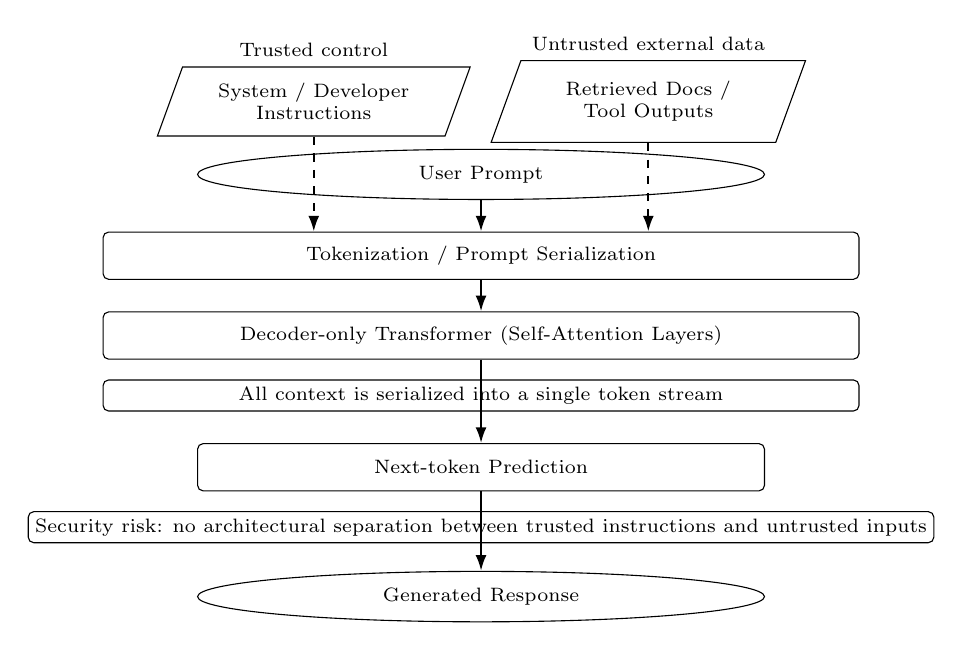
\begin{tikzpicture}[
  font=\scriptsize,
  node distance=4mm and 5mm,
  arrow/.style={-{Latex[length=2mm,width=1.4mm]}, thick},
  dashedarrow/.style={-{Latex[length=2mm,width=1.4mm]}, thick, dashed},
  box/.style={rectangle, rounded corners=2pt, draw, align=center, minimum height=6mm},
  trap/.style={trapezium, trapezium left angle=70, trapezium right angle=110,
               draw, align=center, minimum height=6mm},
  note/.style={rectangle, rounded corners=2pt, draw, align=center, inner sep=2.5pt},
  risk/.style={rectangle, rounded corners=2pt, draw, align=center, inner sep=2.5pt}
]

\node[trap, minimum width=4.0cm] (sys) {System / Developer\\Instructions};
\node[trap, minimum width=4.0cm, right=6mm of sys] (ext) {Retrieved Docs /\\Tool Outputs};

\node[ellipse, draw, align=center, minimum width=7.2cm, minimum height=6mm,
      below=6mm of $(sys)!0.5!(ext)$] (user) {User Prompt};

\node[box, minimum width=9.6cm, below=4mm of user] (ser) {Tokenization / Prompt Serialization};
\node[box, minimum width=9.6cm, below=4mm of ser] (model)
{Decoder-only Transformer (Self-Attention Layers)};
\node[note, minimum width=9.6cm, below=2.5mm of model] (note1)
{All context is serialized into a single token stream};
\node[box, minimum width=7.2cm, below=4mm of note1] (pred) {Next-token Prediction};
\node[risk, minimum width=9.6cm, below=2.5mm of pred] (risk1)
{Security risk: no architectural separation between trusted instructions and untrusted inputs};
\node[ellipse, draw, align=center, minimum width=7.2cm, minimum height=6mm,
      below=3.5mm of risk1] (out) {Generated Response};

\draw[dashedarrow] (sys.south) -- (ser.north -| sys.south);
\draw[dashedarrow] (ext.south) -- (ser.north -| ext.south);

\draw[arrow] (user) -- (ser);
\draw[arrow] (ser) -- (model);
\draw[arrow] (model) -- (pred);
\draw[arrow] (pred) -- (out);

\node[anchor=south] at (sys.north) {Trusted control};
\node[anchor=south] at (ext.north) {Untrusted external data};

\end{tikzpicture}%
}
\caption{Typical LLM application stack. System/developer instructions, user prompts, and retrieved/tool content are serialized into one context, enabling prompt injection and related manipulation.}
\label{fig:llm_stack_attack_surface}
\end{figure}

Across surveys, the most practically exploited threats can be grouped into three categories that align with this stack \cite{c9,c10,c17,c13}:

\textbf{(1) Jailbreak attacks.}
Jailbreaks create prompts to evade safety alignment and obtain policy-violating outputs. Techniques for achieving jailbreaks typically include: role playing, reframing instructions, and optimizing searches for prompts to maximize output \cite{c6,c7,c13}. JailbreakBench is a set of standardized objectives and measures of harmfulness that can be used to measure the effectiveness of a jailbreak and the difficulty of inducing the model to refuse to produce policy-violating outputs in a variety of ways. \cite{c6}.

\textbf{(2) Prompt injection attacks (direct and indirect).}
Prompt injection is an attack on LLM-integrated systems where the input can be in the form of a malicious instruction to the LLM-integrated system via user input (Direct Injection) or via external content retrieved by the system for further processing by the model (Indirect Injection). Prompt injection attacks are capable of overriding system intent, extracting sensitive information embedded in the context, or triggering unwanted or unanticipated behavior by tools used by the application. \cite{c3,c8,c4}. TPrompt injection attacks are particularly relevant to RAG applications as they may embed malicious instructions into benign documents that pass through the upstream filters and retrieval mechanism, and therefore are not detected prior to being processed by the LLM. \cite{c4,c8}.

\textbf{(3) Insecure output handling and downstream exploitation.}
If an application takes model outputs and executes them (as code), renders them (in a browser or web page), or utilizes them as arguments to other tools or functions without proper validation and containment then it is vulnerable to exploitation. . When an application fails to properly handle its model's output, it creates an opportunity for an attacker to execute downstream attacks against the web application such as privilege elevation when model outputs are executed, rendered, or utilized as arguments to other tools or functions. \cite{c12,c11}. As a result, the focus of securing applications using LLMs shifts from filtering prompts to end-to-end application design where the interfaces to tools and sinks for model output are part of the threat surface. \cite{c11}.

\subsection{Scope of This Survey}
\label{subsec:scope}

Additionally, while there are many model-level risks associated with LLMs, including data extraction and model stealing; these types of threats have been identified as lower risk than jailbreaks and prompt injection based on current survey research\cite{c9,c10,c13,c17}. Therefore, this survey will focus on:
(i) Methods that generate and evaluate jailbreak attacks systematically \cite{c6,c7}; (ii) defenses against both prompt- and jailbreak-style manipulation at the prompt, model, and system level; including structured query interfaces, long-context prompt sanitizers, and detection or self-defense mechanisms\cite{c1,c2,c8,c16,c18}. We will consider agential threat models where the use of tools amplify the consequences of manipulating the prompt  \cite{c3,c11}.


%%%%%%%%%%%%%%%%%%%%%%%%%%%%%%%%%%%%%%%%%%%%%%%%%%%%%%%%%%%%%%%%%%%%%%
\section{Literature Review}

This section surveys prior research on the security of large language models (LLMs). To avoid paper-by-paper narration, we organize the literature thematically, emphasizing common attack mechanisms, evaluation practices, defensive strategies, and open challenges.

\subsection{Prompt Injection Attacks}

The reason that adversaries are able to execute prompt injection attacks is due to the fact that in most LLM applications there is no — or very little — separation of instructions and data from untrusted sources. Attackers can, therefore, manipulate the intended functionality of LLMs or can expose sensitive information \cite{c9,c10,c17}. Traditionally, direct prompt injection has been studied as it relates to chat-based environments, where an attacker would embed a malicious instruction(s) within the context of a legitimate user query \cite{c14,c16}.The effectiveness of detection and robustness mechanisms is reduced with the implementation of adaptive paraphrasing and obfuscation techniques that circumvent existing fixed heuristics. \cite{c2,c15,c1}.

\subsection{Jailbreak Attacks and Safety Bypass}

The Jailbreak Attack attempts to use various prompting approaches like Role Play, Persona Switching, and Manipulation of the Instructions to bypass Policy Constraints or Alignment Constraints. \cite{c14,c13}. The JailbreakBench provides a common basis for assessing the success rates for attacks (based on Harmful Goals) and also for Refusal Behaviors (ASRs), so that comparisons across models may be made. \cite{c6}. The most common methods available to Defend against these attacks include: Perturbation Based Robustness, called SMOOTHLLM, Self-Judging Defenses labelled as SelfDefenD, and Explainable Detection, termed JailbreakTracer. Each of these Defenses helps to build greater robustness; however, attackers can still continue to perform Adaptive Search Techniques in order to discover new prompts or new prompt variations through Distribution Shifts\cite{c15,c1,c2}.

\subsection{Indirect Prompt Injection and RAG-Based Threats}

The use of Indirect Prompt Injection creates a larger Attack Surface due to the ability to insert malicious instructions inside third-party content (such as documents that come from a search or from a web page) and provide it to RAGE Pipelines via use of retrieval-augmented-generation techniques. \cite{c4,c3}. Using the spotlight technique, one can illustrate that these attacks succeed regardless of benign user input, which demonstrates the limitations of using only prompt-level filtering \cite{c4}. The use of Defenses has increasingly focused upon protecting the structural separation of Trusted Instructions from Untrusted Input using various means, such as Structured Queries, Sanitization, and Architectural Mediation. \cite{c8,c18,c3}.

\subsection{Agentic LLMs and Tool-Use Vulnerabilities}

When using LLM Systems that operate in Tool-Using Agentic Modes, additional risks exist where an Attacker can extend influence to the Planning of the Attack, the Selection of Tools used in the Attack, and/or the Arguments Provided for those Tools. The result is a significant increase in risk for Unauthorized Action. \cite{c11,c3}. As a result of these phenomena, the Security Problem has transitioned away from being governed by Text Only to now being defined via Control Flow Integrity and Data Flow Integrity, resulting in a call to implement Capability Mediation and Policy-Enforced Tool Invocation.\cite{c3,c11}.

\subsection{Model Misuse and Output-Level Risks}

In addition, generative models can be used by malicious attackers to grow the phishing, human deception, and other cyber abuse industries; furthermore, the methods of injecting jailbreaks or prompts to enhance these models reduce these protections.\cite{c5,c13}. Furthermore, insecure output handling can introduce downstream vulnerabilities to LLM-based applications (such as managing web content and/or application code) when they regard model outputs as trustworthy or reliable code or markup. \cite{c12}.

\subsection{Threat Taxonomy (Summary)}

\begin{table}[H]
\centering
\footnotesize
\setlength{\tabcolsep}{4pt}
\renewcommand{\arraystretch}{1.15}
\caption{Concise taxonomy of key security threats in generative AI systems.}
\label{tab:threat_taxonomy_compact}
\begin{tabularx}{\columnwidth}{@{}p{2.05cm} Y p{2.05cm}@{}}
\toprule
\textbf{Threat} & \textbf{What it exploits / does} & \textbf{Key refs.} \\
\midrule
Direct prompt injection &
User-supplied instructions override intended behavior; may cause leakage or unsafe actions &
\cite{c14,c16,c8} \\
Jailbreak &
Prompt strategies bypass safety/alignment to elicit disallowed outputs &
\cite{c6,c7,c15,c1,c2} \\
Indirect prompt injection (RAG) &
Hidden instructions in retrieved content manipulate generation or actions &
\cite{c4,c3,c18} \\
Agentic/tool misuse &
Multi-step tool invocation enables control/data-flow manipulation and real-world harm &
\cite{c11,c3} \\
Misuse + output risks &
Abuse of model capabilities; unsafe output handling creates downstream vulnerabilities &
\cite{c5,c12} \\
\bottomrule
\end{tabularx}
\end{table}

%%%%%%%%%%%%%%%%%%%%%%%%%%%%%%%%%%%%%%%%%%%%%%%%%%%%%%%%%%%%%%%%%%%%%%
\section{Datasets and Evaluation Benchmarks}

Various Datasets and Benchmarks Commonly Used in the Evaluation of LLM Security. This Overview Highlights The Key Metrics for Each Dataset and The Coverage Gaps Between Datasets Related to Specific LLM Security Threat Surfaces.

\subsection{Jailbreak Benchmarks and Prompt Sets}

JailbreakBench has a set of standardized templates that specify harmful goals and prompts which facilitate the evaluation of jailbreak robustness using ASR/refusal-based metrics in a reproducible manner. \cite{c6}. In addition to providing a common point of reference for jailbreak evaluation, the complementary analyses of adversarial prompt families and automated prompt generation sources (such as distraction) provide valuable insights into attacker methodologies, moving beyond the concept of a static template. \cite{c14,c7}.

\subsection{Detection Datasets}

JailbreakTracer combines real and synthetic jailbreak prompt examples into a dataset that includes explainability labels for each example, thereby creating a supervised detector that works to assist with explanations. \cite{c2}. However, the current state of prompt-only detection datasets generally assumes a direct user/model level interaction and do not capture any potential impacts on the execution of tools or RAG ingestion.

\subsection{Indirect Prompt Injection and Long-Context Evaluation}

Spotlighting offers a unique evaluation scenario to measure the effectiveness of an adversarial instruction embedded within the body of an otherwise benign document when introduced into a RAG pipeline. \cite{c4}. The long-context evaluation scenario will create a need for sanitization-style solutions that can provide a balance between robustness and utility. \cite{c18}.

\subsection{Agentic Evaluation Settings}

Other areas of agentic security focus on evaluating multi-step workflows and measuring both policy violations and unsafe acts that would not be visible in a chat-only evaluation setting. \cite{c11,c3}. A major area not currently addressed is that there are very few standardized datasets and/or metrics that apply to all types of agent implementation

\subsection{Benchmark Comparison (Summary)}

\begin{table}[H]
\centering
\footnotesize
\setlength{\tabcolsep}{4pt}
\renewcommand{\arraystretch}{1.15}
\caption{Concise comparison of security benchmarks and what they cover.}
\label{tab:dataset_comparison_compact}
\begin{tabularx}{\columnwidth}{@{}p{2.05cm} p{1.25cm} p{1.25cm} Y@{}}
\toprule
\textbf{Benchmark} & \textbf{Threat} & \textbf{Setting} & \textbf{Main metric + key limitation} \\
\midrule
JailbreakBench \cite{c6} &
Jailbreak &
Chat &
ASR/refusal; limited coverage of indirect (RAG) and agentic tool-use threats \\
JailbreakTracer \cite{c2} &
Detection &
Chat &
Detection accuracy/labels; prompt-only, not tool/RAG execution \\
Spotlighting eval \cite{c4} &
Indirect PI &
RAG &
Injection success; often single-step, limited agentic realism \\
PISanitizer eval \cite{c18} &
PI (long ctx) &
Chat/RAG &
Injection success + utility trade-off; may not cover tool misuse \\
Agentic suites \cite{c11,c3} &
Agentic &
Agent &
Policy violations/task safety; no universal dataset/metrics across agents \\
\bottomrule
\end{tabularx}
\end{table}

\subsection{Evaluation Gaps}

The predominant metrics used in current evaluate are that of chat-only jailbreak scenario settings and refusals/ASR. \cite{c6,c13,c17}. Even though it is currently possible to directly exploit both prompt injection and long-context behaviour, comparative benchmarks are much less consistently available. \cite{c4,c18}. Agentic (intervention-based) systems have increased the threat surface, but there is limited availability of standardised data sets and comparable safety measures regarding their integrity when utilising tools. \cite{c11,c3}.

%%%%%%%%%%%%%%%%%%%%%%%%%%%%%%%%%%%%%%%%%%%%%%%%%%%%%%%%%%%%%%%%%%%%%%
\section{Defense Mechanisms}
Defenses against prompt injection and model misuse must be multi-layered throughout generative AI’s various components. Empirical evidence continues to show that having a singular line of defense is not enough against opportunistically evolving adversaries, which has led to a shift toward a multi-layered defence approach.  

\subsection{Defense Taxonomy}

\textbf{Prompt-level defenses} A prompt can be examined through a variety of heuristics and classification techniques or structured and partially processed Queries as well as sanitized prompts. These approaches can typically be successfully challenged through Paraphrasing (to obscure intent), Distracting (to redirect attention), and/or through Indirect Injection Attacks (to inject content into Prompts or queries without direct access to the system). As such, even though these are lighter-weight, easy-to-replicate methods, they remain continuously adaptable by adversarial actors  \cite{c6,c7,c8,c13,c14,c18}.

\noindent\textbf{Output-level defenses}  Where generating outputs against safe use policies can be managed at the point of output checking or moderation; this approach has been widely used but is not an appropriate method for Agentically produced outputs where the possibility of generating unsafe behaviour exists prior to the application of an Output filter.  \cite{c9,c10,c12}.

\noindent\textbf{Model-centric defenses}  Through the integration of Alignment Objectives,1 Agent-Based system training such as Instruction Tuning; training the model through the injection of “adversarial” input (Adversarial Training) to improve performance against known “jailbreaks”; incorporating formulating an agent by limiting how far the agent moves out of alignment to observed behaviour through Decoding Constraints; and using concepts from Reinforcement Learning. These approaches will improve the robustness of models against known jailbreaks but can also leave them vulnerable to novel Indirect or Bypass attacks and can have a major negative effect on overall model utility as a result of Over-Refusal. \cite{c13,c15,c1}.

\noindent\textbf{Ensemble-based defenses}  An Ensemble Approach will result in a greater amount of latency and processing effort, but will generate better defence against attacks by having multiple models judge the safety of Prompts or Outputs.  \cite{c6,c15,c1}.

\noindent\textbf{System-level defenses}  When managing how Tools will be used in an Agentic environment, Managing Tool Usage and Privileges can best be achieved through the use of Capability Controls, Sandboxing, and Policy Governing Execution at the System Level.  \cite{c11,c3,c4}.

%%%%%%%%%%%%%%%%%%%%%%%%%%%%%%%%%%%%%%%%%%%%%%%%%%%%%%%%%%%%%%%%%%%%%%
\section{Open Challenges and Future Directions}

Although a considerable amount of progress has been made in securing generative AI systems, challenges remain as generative models are being introduced into complex pipelines using long-context strategies and tool using agents. 
Some areas of emerging research based on the results of recent attacker and defender work and gaps in evaluation are identified below: 

\subsection{Adaptive and Automated Adversaries}

Some types of defences work for certain fixed prompt sets. But when it comes to defences against adaptive adversaries, they do not perform as well because the malicious entity is able to continually find ways to affect the and test the resilience of your deployed security. 
This has been highlighted through studies on the rapid development of automated jail breaking of generative AI and the exponential threats arising from optimizing prompt to generate every possible version of any text query. 
Future work would need to include the evaluation of available defence strategies under evolving feedback from the iterations of attacks, multiple languages, transfer across domains, and multi-step interactions where attacks come in stages with a consequence to change how the Models behave, as highlighted in prior studies  \cite{c14,c3}.

\subsection{Realistic Evaluation Beyond Static Prompt Sets}

Benchmarking is not a sufficient means of evaluating systems. Benchmarks tend to focus on producing a single-turn prompt set and generating a summary, but most deployments of generative AIs provide either resource aggregation and long-context systems, and also utilise agent actions. Risk assessment in this scenario is based on not just the text it generates, but also the downstream impact it generates in the network of other actions it subsequently performs (e.g. calling tools, accessing data, and executing action steps)  \cite{c11,c3}.

The design of benchmarks should include untrusted input channels (e.g. documents and web pages), and attempt to be able to quantify the complete system risk of any new type of generative AI.  \cite{c4,c6}.

\subsection{Evaluation Metrics Beyond ASR and Refusal Rates}

ASR (Automated Segmentation, Recognition) is a widely used tool, but it can hide smaller problems (such as accidentally leaking sensitive info by accident) and at other times make safety look better than it is, as when a model is trained to reject requests based on brittle/irregular responses. 
Refusal based scoring is ineffective at capturing how risky individual actions are when working with agents. 
To improve future evaluations of ASRs, we should combine (i) detailed harm metrics, (ii) utility preservation, (iii) safety of actions associated with tools, and (iv) comparison-based calibration of results against a specific human evaluation based on the representative population of ASR agents. \cite{c11,c3}.

Future evaluation should combine (i) graded harm metrics, (ii) utility preservation, (iii) action safety for tool use, and (iv) calibration against human evaluation on representative subsets \cite{c6,c17}.

% ---------------------------------------------------------
% TABLE INSERTED HERE
% ---------------------------------------------------------
\begin{table}[h]
\centering
\caption{Comparison of Evaluation Dimensions in AI Safety Benchmarks}
\begin{tabular}{|p{3cm}|p{4.5cm}|}
\hline
\textbf{Metric} & \textbf{Description} \\ \hline
Attack Success Rate (ASR) & Measures percentage of successful jailbreaks but may hide partial harms. \\ \hline
Utility Preservation & Ensures model remains useful while being robust to attacks. \\ \hline
Action-Level Safety & Evaluates risk when models perform actions via tools or agents. \\ \hline
Human Calibration & Benchmarks aligned with expert evaluation for nuanced harm scoring. \\ \hline
\end{tabular}
\label{tab:evaluation_comparison}
\end{table}
% ---------------------------------------------------------

\subsection{Securing Agentic Systems and Tool Use}

When LLMs are utilized as an agentic tool, prompt injection creates a systemic security threat in addition to being a purely linguistic issue. 
This type of deployment can result in control-flow failures and data-flow failures that are open to exploitation by attackers in order to achieve unauthorized actions.  \cite{c11,c3}.

One path forward for addressing this type of problem is to create a structure that clearly delineates; therefore, 'Principled Containment' would include using the least privilege to access tools, specifying that agents must go through an explicit authorization process in order to utilize these tools, and instituting a Policy i.e., containing the effect of tools on agents, even when an agent-model is only partially compromised.  \cite{c3}.

\subsection{Defenses for Indirect Prompt Injection and Untrusted Data}

While structuring and separating context can limit the risk of indirect prompt injection, attackers may utilise similar structural formats to exploit weaknesses  \cite{c4}.

Innovative approaches include creating structured interfaces with robust provenance-aware context building and providing system-level mediation   \cite{c8,c4}.

\subsection{Long-Context and RAG Sanitization}

Long-context and retrieval augmented generation (RAG) pipelines increase an adversary's ability to embed an instruction or a "prompt" deep into the retrieved content. When using short-context defence mechanisms, many of them dramatically decrease in effectiveness when faced with adversarial spans that are both sparse and buried. 

Prompt sanitisation approaches that have been developed specifically for long-context organisations provide an avenue of defence, but how to effectively defend against evolutionarily adapting adversaries remains an unopened question.  \cite{c18}.

\subsection{Defense-in-Depth and Practical Deployability}

There isn’t one defense strategy fitting to every Threat Class. 

In order to provide real Security, a Multi-Layered Defense Architecture, which incorporates pre-inference Controls, Post-Inference decoding Robustness, Rendering Checks and System Containment Levels must be established. 

 

Oftentimes, a challenge remains constant in attempting to deploy Defenses under Latency and Cost Constraints; when using a Black-Box API, it may even be impossible to perform Internal Training or Internal Instrumentation.  \cite{c17,c10}.

\subsection{Reproducibility and Standard Reporting}

In summary, more robust norms for research reproducibility should be established within the community. This includes comprehensive descriptions of threat models, prompt templates, attacker resources available for exploiting vulnerabilities and scenarios whereby systems would fail. 

 

By providing clear guidelines for how to evaluate results and utilizing defined evaluation harnesses, it will be possible to easily determine the strength of multiple, disparate studies, thereby reducing the likelihood of overfitting based upon a small, narrow set of prompts.  \cite{c6,c17}.


% ==========================================================
\section{State-of-the-Art Defense Mechanisms}
\label{sec:sota_defenses}
% ==========================================================

The majority of recent studies in regards to LLM security have focused on developing multi-layered defense strategies for the prompts, models, systems and will utilize a combination of detection, structural isolation, and capability controls to prevent jailbreak and prompt injection attacks under realistic operational conditions. 

% ==========================================================
\subsection{Defense Taxonomy and Design Dimensions}
\label{subsec:defense_taxonomy}
% ==========================================================

Table~\ref{tab:defense_taxonomy} summarizes representative defense paradigms, highlighting where each mechanism intervenes and the threats it primarily addresses.
\subsection{Defense Taxonomy and Design Dimensions}
\label{subsec:defense_taxonomy}

% Flush any previous floats so they don't jump ahead and steal space
\FloatBarrier

\noindent\begin{minipage}{\columnwidth}
\centering
\small
\setlength{\tabcolsep}{4pt}
\renewcommand{\arraystretch}{1.15}
\captionsetup{type=table}
\caption{Taxonomy of representative LLM security defenses.}
\label{tab:defense_taxonomy}
\begin{tabularx}{\columnwidth}{@{}p{2.25cm} Y p{2.15cm}@{}}
\toprule
\textbf{Defense Class} & \textbf{Core Mechanism} & \textbf{Representative Works} \\
\midrule
Prompt-side detection &
Classify/score inputs for jailbreak or injection risk before generation &
JailbreakTracer~\cite{c2}, SmoothLLM~\cite{c15} \\
Prompt isolation &
Structurally separate trusted instructions from untrusted content &
StruQ~\cite{c8}, Spotlighting~\cite{c4} \\
Model-level self-defense &
Secondary model evaluates/vetoes unsafe generations &
SelfDefend~\cite{c1} \\
System-level capability control &
Least-privilege execution; constrained tool use and data access &
CaMeL~\cite{c3}, Agentic security~\cite{c11} \\
\bottomrule
\end{tabularx}
\end{minipage}

% Prevent following figures from floating above this subsection
\FloatBarrier


These approaches are complementary rather than mutually exclusive, and recent systems increasingly integrate multiple layers into a single defense stack.

% ==========================================================
\subsection{Model-Level Self-Defense: SELFDEFEND}
\label{subsec:selfdefend}
% ==========================================================

The SelfDefend architecture [1] utilizes an architecture referred to as Dual-LLM Shadow Execution; where an adversary's LLM creates responses in parallel with a Defense LLM that identifies potential "harmful" intent within the prompt given to the adversary and intermediate output generated by the adversary. If the Defense LLM determines that the response created by the adversary does not pose a risk, then the response will be released. However, if the Defense LLM determines that the response created by the adversary is potentially malicious, the response will either be rejected or replaced with a denial/refusal.

Across various types of jailbreak families, substantial reductions in Attack Success Rate (ASR) were demonstrated while only slight degradation was observed on benign prompts. Therefore, these results demonstrate the feasibility of model-level self monitoring without altering the base model weight values [1].

 

\begin{figure}[t]
\centering
\resizebox{0.9\columnwidth}{!}{%
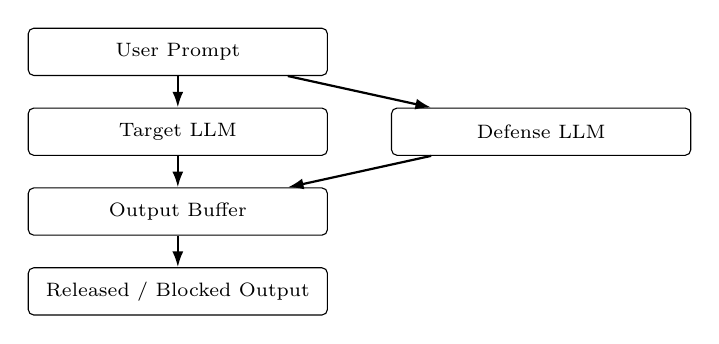
\begin{tikzpicture}[
  font=\scriptsize,
  box/.style={draw, rounded corners=2pt, align=center, minimum height=6mm},
  arrow/.style={-{Latex[length=2mm,width=1.4mm]}, thick}
]
\node[box, minimum width=3.8cm] (prompt) {User Prompt};
\node[box, below=4mm of prompt, minimum width=3.8cm] (target) {Target LLM};
\node[box, right=8mm of target, minimum width=3.8cm] (defense) {Defense LLM};
\node[box, below=4mm of target, minimum width=3.8cm] (buffer) {Output Buffer};
\node[box, below=4mm of buffer, minimum width=3.8cm] (final) {Released / Blocked Output};

\draw[arrow] (prompt) -- (target);
\draw[arrow] (prompt) -- (defense);
\draw[arrow] (target) -- (buffer);
\draw[arrow] (defense) -- (buffer);
\draw[arrow] (buffer) -- (final);
\end{tikzpicture}
}
\caption{SELFDEFEND dual-LLM shadow execution. A defense model evaluates risk before outputs are released.}
\label{fig:selfdefend_arch}
\end{figure}.

% ==========================================================
\subsection{Prompt Isolation and Structured Pipelines}
\label{subsec:spotlighting}
% ==========================================================

Techniques utilizing prompt isolation are intended to prevent Instruction Override through the separation of trusted Control Signals from Untrusted Content. Techniques such as Spotlighting [4] and StruQ [8], utilize structured query formats and real-time screening to restrict how User Inputs and Retrieved Documents affect Generation.

Significant reduction in Indirect Prompt Injection has been demonstrated in RAG-based applications through the enforcement of structured query formats and real-time screening; preventing hidden instructions contained within Retrieved Documents from overriding System Intent [4, 8].

 

\begin{figure}[t]
\centering
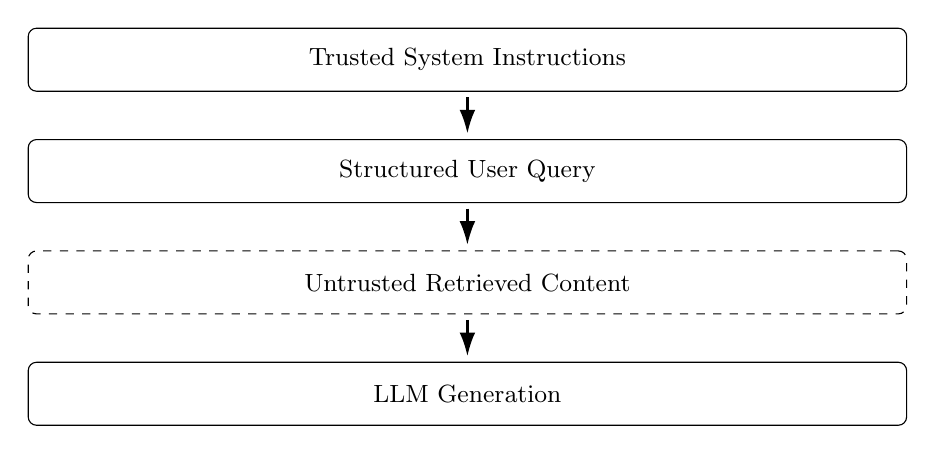
\begin{tikzpicture}[
  font=\small,
  box/.style={
    draw,
    rounded corners=3pt,
    minimum width=0.92\columnwidth,
    minimum height=8mm,
    align=center
  },
  dashedbox/.style={
    draw,
    dashed,
    rounded corners=3pt,
    minimum width=0.92\columnwidth,
    minimum height=8mm,
    align=center
  },
  arr/.style={-{Latex[length=3mm,width=2mm]}, thick}
]

\node[box] (sys) {Trusted System Instructions};
\node[box, below=6mm of sys] (query) {Structured User Query};
\node[dashedbox, below=6mm of query] (retrieved) {Untrusted Retrieved Content};
\node[box, below=6mm of retrieved] (gen) {LLM Generation};

% Draw three short arrows (never through text)
\draw[arr, shorten <=2pt, shorten >=2pt] (sys.south) -- (query.north);
\draw[arr, shorten <=2pt, shorten >=2pt] (query.south) -- (retrieved.north);
\draw[arr, shorten <=2pt, shorten >=2pt] (retrieved.south) -- (gen.north);

\end{tikzpicture}
\caption{Prompt isolation via structured pipelines. Trusted instructions are kept separate from untrusted retrieved content before generation.}
\label{fig:structured_prompt_isolation_v2}
\end{figure}

\caption{Prompt isolation via structured pipelines.}
\label{fig:structured_prompt_isolation}
\end{figure}

\caption{Prompt isolation via structured pipelines. Trusted instructions and structured queries are separated from untrusted retrieved content before LLM generation.}
\label{fig:structured_prompt_isolation}
\end{figure}

\caption{Prompt isolation via structured pipelines. Trusted instructions are kept distinct from untrusted retrieved content.}
\label{fig:spotlighting_arch}
\end{figure}


% ==========================================================
\subsection{Prompt-Side Detection: JailbreakTracer and Related Methods}
\label{subsec:jailbreaktracer}
% ==========================================================

One approach of defending against prompt-side vulnerabilities would be to identify malicious intent prior to generation; JailbreakTracer ~\cite{c2} employs this methodology using transformer- based classifiers trained on curated and synthetically augmented datasets for detecting jailbreak attempts, while providing interpretable risk score assignments for each attempt. The graded response capabilities in detecting jailbreak attempts enables the use of responses ranging from refusal to output sanitization, as well as escalation of the response to stricter defenses, as opposed to the binary filtering capability of other methods. The speed and reliability of detection-based methods are generally very fast and effective when combined with a downstream strategy for containment. ~\cite{c13,c15}.

% ==========================================================
\subsection{System-Level Defenses for Agentic LLMs}
\label{subsec:camel}
% ==========================================================

The partnership between LLM and an untrusted data source is managed through a quaran- tine model using CaMeL ~\cite{c3} .The architecture uses a privileged planning (LLM) layer to coordinate activ- ities, while also ensuring that any untrusted content is routed to the interpreter for enforceable policy execution. This prevents untrusted content from directly affecting the actions of the LLM. In an absolute sense, these types of systems have become even more important in the agency environment where tool use has the potential to greatly amplify the effects of prompt manipulation in the world outside the toolkit. ~\cite{c11}.

% ==========================================================
\subsection{Summary and Open Challenges}
\label{subsec:summary_defenses}
% ==========================================================

While state of the art defenses have demonstrated that defense in depth is required to effectively mitigate jailbreak and prompt injection attacks, we believe that there are still many open issues that require attention. The ability to adapt to adaptive attackers will remain a challenge to address, evaluation in long context settings will also continue to pose an open challenge, and finally the trade off between performance/usability and security remains an open issue.

 

%%%%%%%%%%%%%%%%%%%%%%%%%%%%%%%%%%%%%%%%%%%%%%%%%%%%%%%%%%%%%%%%%%%%%%
\section{Conclusion}
\label{sec:conclusion}

Generative AI systems and LLM-based applications deliver strong capabilities but also introduce new security failure modes because natural-language prompting simultaneously serves as \emph{control} and \emph{data}. This survey organized the literature around three practically exploited threat families---jailbreaks, direct/indirect prompt injection (especially under RAG), and misuse or insecure output handling---and highlighted how these risks intensify in agentic settings where models can invoke tools and trigger real-world side effects \cite{c6,c9,c10,c11,c13,c12}.

Across the reviewed works, a consistent empirical theme is that \emph{single-stage defenses are brittle} under adaptive prompting and distribution shift, motivating defense-in-depth stacks that combine (i) prompt-side risk detection \cite{c2,c15}, (ii) architectural separation and structured prompting to reduce instruction override, particularly for indirect injection \cite{c4,c8,c18}, (iii) model-level self-monitoring/gating \cite{c1}, and (iv) system-level capability mediation and least-privilege tool execution for agentic pipelines \cite{c3,c11}. Benchmarks and evaluation suites further indicate that refusal/ASR-only reporting is insufficient for deployed systems, and should be complemented with utility preservation, action-level safety, and calibration against human judgment \cite{c6,c11,c13,c17}.

\begin{table}[t]
\centering
\footnotesize
\setlength{\tabcolsep}{4pt}
\renewcommand{\arraystretch}{1.15}
\caption{Defense-in-depth layers for deployed LLM systems (representative examples).}
\label{tab:conclusion_layers}
\begin{tabularx}{\columnwidth}{@{}p{2.25cm}Yp{2.1cm}@{}}
\toprule
\textbf{Layer} & \textbf{Goal in practice} & \textbf{Examples} \\
\midrule
Prompt-side screening & Detect/score jailbreak or injection intent before generation & JailbreakTracer \cite{c2}, SmoothLLM \cite{c15} \\
Prompt isolation & Separate trusted instructions from untrusted user/retrieved content; constrain influence & Spotlighting \cite{c4}, StruQ \cite{c8}, long-context sanitization \cite{c18} \\
Model-level gating & Shadow execution / secondary judging to block unsafe generations & SelfDefend \cite{c1} \\
System-level control & Enforce capability mediation, least privilege, and policy-checked tool use & CaMeL \cite{c3}, agentic mitigation \cite{c11} \\
\bottomrule
\end{tabularx}
\end{table}

\begin{figure}[t]
\centering
\resizebox{0.95\columnwidth}{!}{%
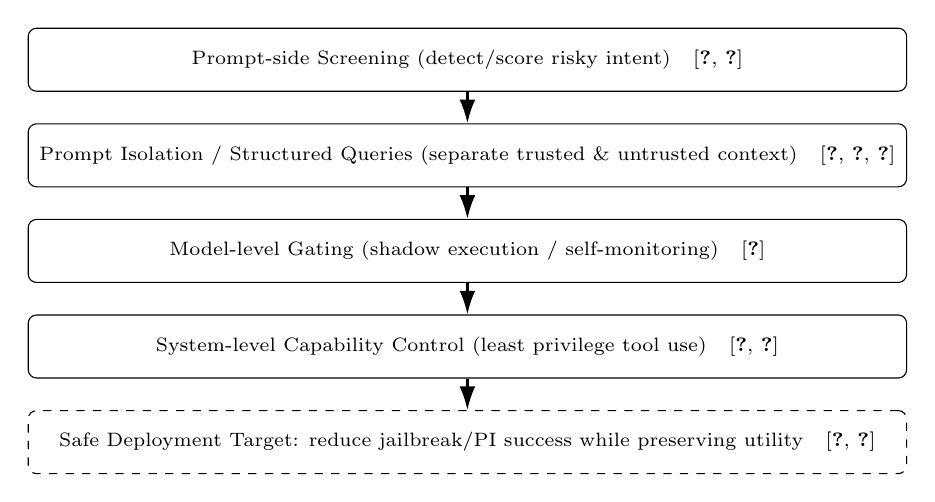
\begin{tikzpicture}[
  font=\scriptsize,
  box/.style={draw, rounded corners=3pt, align=center, minimum width=0.92\columnwidth, minimum height=8mm},
  dashedbox/.style={draw, dashed, rounded corners=3pt, align=center, minimum width=0.92\columnwidth, minimum height=8mm},
  arr/.style={-{Latex[length=3mm,width=2mm]}, thick}
]
\node[box] (l1) {Prompt-side Screening (detect/score risky intent) \ \ \cite{c2,c15}};
\node[box, below=4mm of l1] (l2) {Prompt Isolation / Structured Queries (separate trusted \& untrusted context) \ \ \cite{c4,c8,c18}};
\node[box, below=4mm of l2] (l3) {Model-level Gating (shadow execution / self-monitoring) \ \ \cite{c1}};
\node[box, below=4mm of l3] (l4) {System-level Capability Control (least privilege tool use) \ \ \cite{c3,c11}};
\node[dashedbox, below=4mm of l4] (out) {Safe Deployment Target: reduce jailbreak/PI success while preserving utility \ \ \cite{c6,c17}};
\draw[arr] (l1) -- (l2);
\draw[arr] (l2) -- (l3);
\draw[arr] (l3) -- (l4);
\draw[arr] (l4) -- (out);
\end{tikzpicture}%
}
\caption{A practical defense-in-depth view: combining detection, structural isolation, gating, and capability control yields stronger robustness than any single layer.}
\label{fig:defense_in_depth_conclusion}
\end{figure}

Finally, several open problems remain. First, defenses must be stress-tested against adaptive, automated attackers and long-context settings that hide sparse malicious spans \cite{c7,c18}. Second, evaluation should move beyond static prompts toward end-to-end measurements that incorporate tool actions, downstream execution, and realistic deployment constraints \cite{c11,c12,c17}. Third, practitioners must balance security with usability, latency, and cost, especially when models are accessed through black-box APIs \cite{c10,c17}. Addressing these challenges will require composable architectures, standardized reporting practices, and continually updated benchmarks that reflect both emerging attacks and real-world agentic workloads \cite{c6,c11,c17}.


%%%%%%%%%%%%%%%%%%%%%%%%%%%%%%%%%%%%%%%%%%%%%%%%%%%%%%%%%%%%%%%%%%%%%%
\begin{thebibliography}{99}

\bibitem{c1}
Wang, X., Wu, D., Ji, Z., Li, Z., Ma, P., Wang, S., et al.
\newblock \emph{SelfDefend: LLMs Can Defend Themselves against Jailbreaking in a Practical Manner}.
\newblock arXiv preprint arXiv:2406.05498, 2024.

\bibitem{c2}
Abdullah, F., Raihan, M., Rahman, A., et al.
\newblock \emph{JailbreakTracer: Explainable Detection of Jailbreaking Prompts in Large Language Models Using Synthetic Data Generation}.
\newblock IEEE Transactions on Information Forensics and Security, 2025.

\bibitem{c3}
Dvijotham, K., et al.
\newblock \emph{Defeating Prompt Injections by Design: CaMeL---A Capability-Mediated LLM Architecture}.
\newblock arXiv preprint arXiv:2503.18813, 2025.

\bibitem{c4}
Hines, K., Lopez, G., Hall, M., Zarfati, F., Zunger, Y., K{\i}c{\i}man, E.
\newblock \emph{Defending Against Indirect Prompt Injection Attacks with Spotlighting}.
\newblock arXiv preprint arXiv:2403.14720, 2024.

\bibitem{c5}
Gupta, M., Akiri, C., Aryal, K., Parker, E., Praharaj, L.
\newblock \emph{From ChatGPT to ThreatGPT: Impact of Generative AI in Cybersecurity and Privacy}.
\newblock IEEE Transactions on Dependable and Secure Computing, 2023.

\bibitem{c6}
Liu, Y., Li, M., Zhang, X., et al.
\newblock \emph{JailbreakBench: An Open Robustness Benchmark for Jailbreaking Large Language Models}.
\newblock arXiv preprint arXiv:2404.01318, 2024.

\bibitem{c7}
Zhang, Y., Sun, H., Chen, Z., et al.
\newblock \emph{Distract Large Language Models for Automatic Jailbreak Attack}.
\newblock In Proceedings of EMNLP 2024, 2024.

\bibitem{c8}
Wang, R., Liu, X., Xu, Z., et al.
\newblock \emph{StruQ: Defending Against Prompt Injection with Structured Queries}.
\newblock OpenReview, 2024.

\bibitem{c9}
Li, J., Chen, Y., Wang, S., et al.
\newblock \emph{A Survey on Large Language Model Security and Privacy: The Good, The Bad, and The Ugly}.
\newblock Pattern Recognition Letters, 2024.

\bibitem{c10}
Sikdar, B.
\newblock \emph{Privacy and Security Concerns in Generative AI: A Comprehensive Survey}.
\newblock IEEE Access, 2024.

\bibitem{c11}
Zhao, T., Huang, Q., Xu, Y., et al.
\newblock \emph{Securing Agentic AI: A Comprehensive Threat Model and Mitigation Framework for Generative AI Agents}.
\newblock arXiv preprint arXiv:2504.19956, 2025.

\bibitem{c12}
Kumar, S., Verma, A., Gupta, N.
\newblock \emph{Insecure Output Handling in Large Language Models and Approaches to Enhance Output Security}.
\newblock TechRxiv, 2024.

\bibitem{c13}
Zhou, H., Liu, J., Wang, P., et al.
\newblock \emph{Jailbreaking and Mitigation of Vulnerabilities in Large Language Models}.
\newblock arXiv preprint arXiv:2410.15236, 2024.

\bibitem{c14}
Wei, J., Yu, Z., Chen, X., et al.
\newblock \emph{Don’t Listen To Me: Understanding and Exploring Jailbreak Prompts of Large Language Models}.
\newblock arXiv preprint arXiv:2403.17336, 2024.

\bibitem{c15}
Robey, A., Hassidim, A., Singh, A., et al.
\newblock \emph{SMOOTHLLM: Defending Large Language Models Against Jailbreaking Attacks}.
\newblock arXiv preprint arXiv:2310.03684, 2023.

\bibitem{c16}
Chen, Y., Liu, S., Zhang, R., et al.
\newblock \emph{Defense Against Prompt Injection Attack by Leveraging Attack Techniques}.
\newblock In Proceedings of ACL 2025, 2025.

\bibitem{c17}
Sikdar, B.
\newblock \emph{Security Concerns for Large Language Models: A Survey}.
\newblock arXiv preprint arXiv:2505.18889, 2025.

\bibitem{c18}
Wang, L., Xu, Y., Zhou, K., et al.
\newblock \emph{PISanitizer: Preventing Prompt Injection to Long-Context LLMs via Prompt Sanitization}.
\newblock arXiv preprint arXiv:2511.10720, 2025.

\end{thebibliography}

\end{document}
